\subsection{Pegeldiagram}
\label{sec:Pegeldiagram}

Nachfolgend sind in den Abbildungen \ref{pic:Pegeldiagram_Line} und \ref{pic:Pegeldiagram_Ext} die Pegeldiagramme des Signalpfades dargestellt.
Von Line IN können Signale mit bis zu +6 \si{dBV} ankommen. Mit einem 1:1 Spannungsteiler wird das Signal auf 0 \si{dBV} abgeschwächt.

\begin{figure}[H]
	\centering
	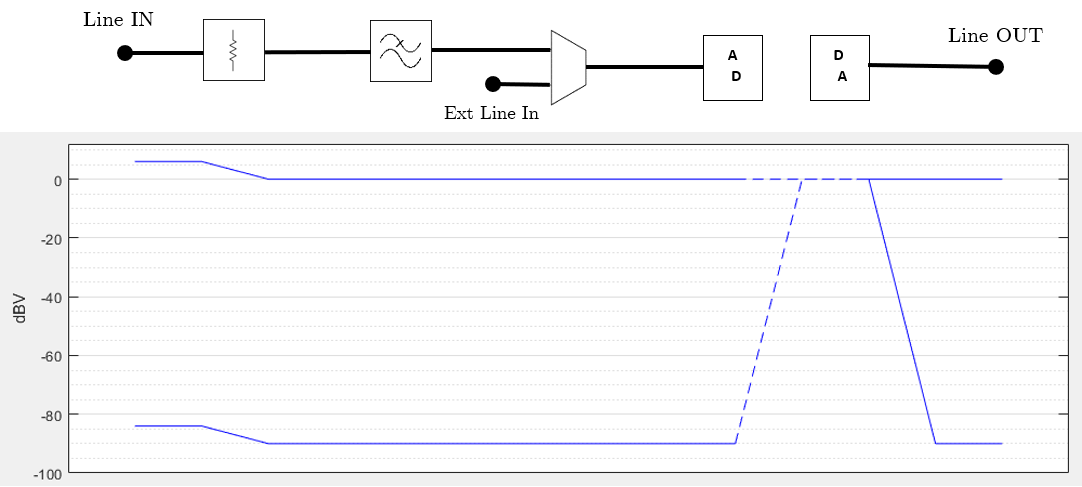
\includegraphics[width=1.0\linewidth]{level_diagram_line}
	\caption{Pegeldiagram des Audiopfades von Line IN nach Line OUT}
	\label{pic:Pegeldiagram_Line}
\end{figure}

\todo{SB - Ausgangspegel +6dB bis -40.5 dB (-34.5 -6)}

\begin{figure}[H]
	\centering
	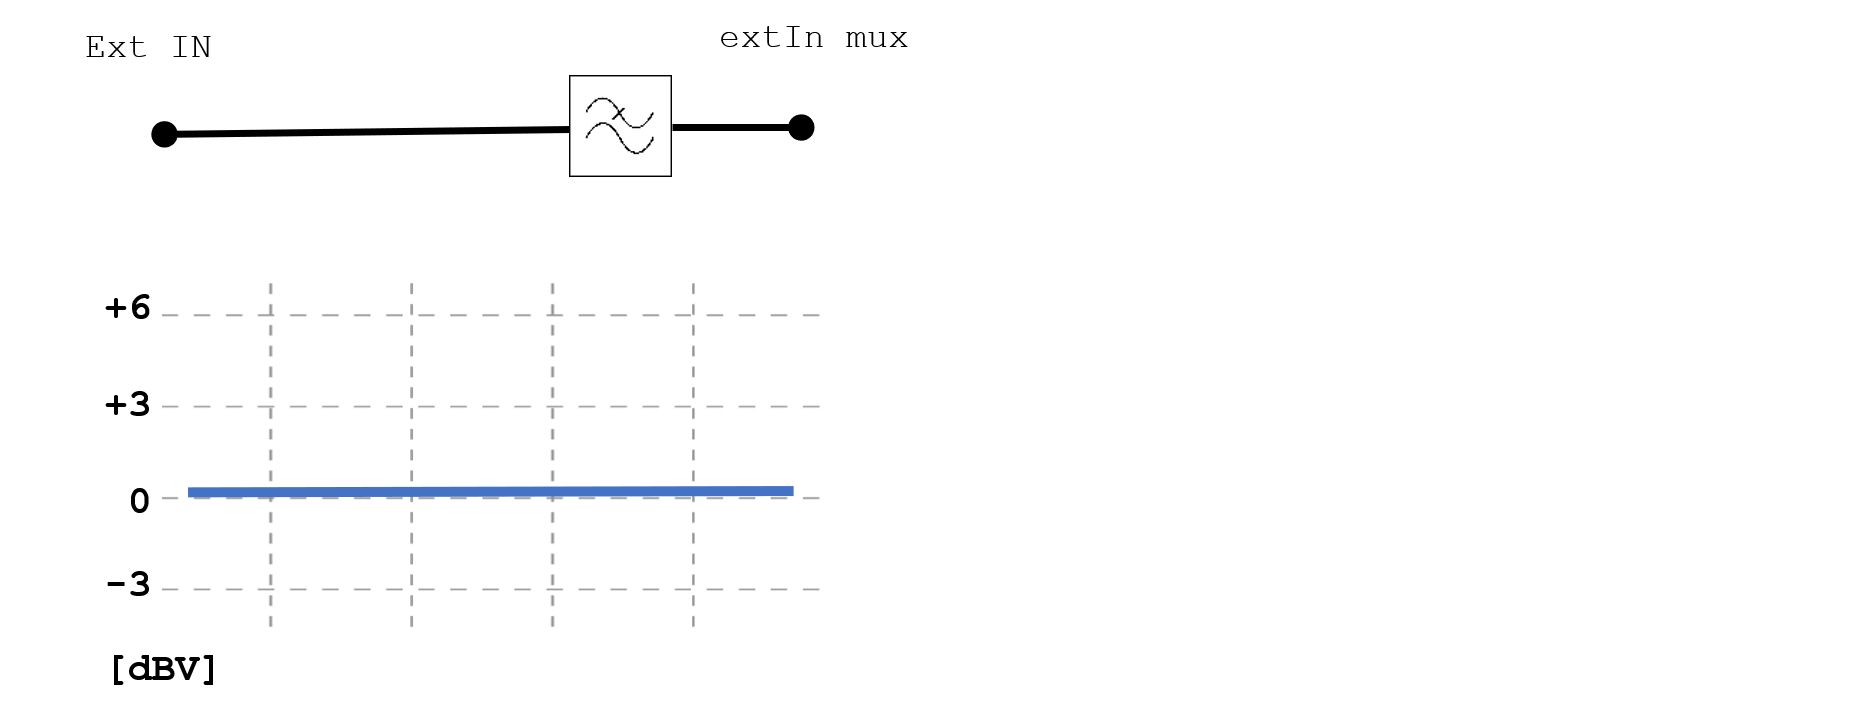
\includegraphics[width=1.0\linewidth]{level_diagram_ext}
	\caption{Pegeldiagram des Audiopfades von Ext IN bis zum Audio Switch}
	\label{pic:Pegeldiagram_Ext}
\end{figure}

